\hyperdef{}{tilda}{}

\subsection{Sequenzalinierung in Python}

\subsubsection{\texorpdfstring{{Allgemeine
Strategien}}{Allgemeine Strategien}}

\par\noindent\textbf{Python und JavaScript}

Python und JavaScript sind sich im Prinzip recht ähnlich, was die
Datentypen anbelangt. Wir werden auch für unsere Python-Implementierung
auf Listen (Arrays in JavaScript) zurückgreifen, und Loops durchführen
(\textbf{while} für den Traceback und \textbf{for} für die
Matritzen-Füllung). Allerdings können wir in Python kompakter
formulieren und haben es daher etwas leichter, den Kode aufzusetzen.




\par\noindent\textbf{Struktur}

Die Implementierung des Alinierungsalgorithmus in Python (eine Version
des \href{http://bibliography.lingpy.org?key=Wagner1974}{Wagner-Fischer
Algorithmus}) basiert auf den gleichen Blöcken, wie auch die Alinierung
in der JavaScript-Implementierung, die wir in der vorigen Sitzung
besprochen haben:

\begin{enumerate}
\itemsep1pt\parskip0pt\parsep0pt
\item
  Vorbereitung von Konstanten und allgemeine Checks
\item
  Initialisierung von Matrix und Traceback
\item
  Ausfüllen von Matrix und Traceback
\item
  Traceback und Konstruktion der Alinierungen
\end{enumerate}




\par\noindent\textbf{Dann kann's ja losgehen!}

Genau! Denn der Algorithmus ist tatsächlich sehr leicht in Python zu
implementieren, vorausgesetzt man ist mit den Datentypen ein wenig
vertraut. Aber wir schauen uns das jetzt Schritt für Schritt in Ruhe an.



\subsubsection{Implementierung der Matrixberechnung}

\par\noindent\textbf{Grundlegender Aufbau}

\begin{verbatim}

def wf_align(seqA, seqB):
    """
    BLABLABLE
    """

    # Vorgeplänkel
    # Initialisierung von Matrix und Traceback
    # Ausfüllen von Matrix und Traceback
    # Traceback-Vorbereitung
    # Traceback
    # Traceback-Nachbereitung

    return almA, almB, ED
\end{verbatim}





\par\noindent\textbf{Vorgeplänkel}

\begin{verbatim}
def wf_align(seqA, seqB):
    """
    Align two sequences using the Wagner-Fisher algorithm.
    """

    # check for empty seqs
    if not seqA or not seqB:
        return

    # store length of sequences
    m = len(seqA)+1
    n = len(seqB)+1

    # Initialisierung von Matrix und Traceback
    # Ausfüllen von Matrix und Traceback
    # Traceback-Vorbereitung
    # Traceback
    # Traceback-Nachbereitung

    return almA, almB, ED
\end{verbatim}





\par\noindent\textbf{Initialisierung von Matrix und Traceback}

\begin{verbatim}
def wf_align(seqA, seqB):
    """
    Align two sequences using the Wagner-Fisher algorithm.
    """
    # Vorgeplänkel
    # Initialisierung von Matrix und Traceback
    M = [[0 for i in range(n)] for j in range(m)]
    T = [[0 for i in range(n)] for j in range(m)]

    # initialize M and T
    for i in range(m): 
        M[i][0] = i
    for i in range(n):
        M[0][i] = i
    for i in range(1,m):
        T[i][0] = 1
    for i in range(1,n):
        T[0][i] = 2

    # Ausfüllen von Matrix und Traceback
    # Traceback-Vorbereitung
    # Traceback
    # Traceback-Nachbereitung

    return almA, almB, ED
\end{verbatim}





\par\noindent\textbf{Ausfüllen von Matrix und Traceback}

\begin{verbatim}
def wf_align(seqA, seqB):
    """
    Align two sequences using the Wagner-Fisher algorithm.
    """
    # Vorgeplänkel
    # Initialisierung von Matrix und Traceback
    # Ausfüllen von Matrix und Traceback

    # start the main loop
    for i in range(1,m):
        for j in range(1,n):

            # get the chars
            charA = seqA[i-1]
            charB = seqB[j-1]

            # check identity
            if charA == charB:
                match = M[i-1][j-1]
            else:
                match = M[i-1][j-1] + 1

            # get the gaps
            gapA = M[i-1][j] + 1
            gapB = M[i][j-1] + 1

            # compare the stuff
            if match <= gapA and match <= gapB:
                M[i][j] = match
            elif gapA <= gapB:
                M[i][j] = gapA
                T[i][j] = 1 # don't forget the traceback
            else:
                M[i][j] = gapB
                T[i][j] = 2 # don't forget the traceback

    # Traceback-Vorbereitung
    # Traceback
    # Traceback-Nachbereitung

    return almA, almB, ED
\end{verbatim}



\subsubsection{\texorpdfstring{{Implementierung des
Traceback}}{Implementierung des Traceback}}

\par\noindent\textbf{Traceback-Vorbereitung}

\begin{verbatim}
def wf_align(seqA, seqB):
    """
    Align two sequences using the Wagner-Fisher algorithm.
    """
    # Vorgeplänkel
    # Initialisierung von Matrix und Traceback
    # Ausfüllen von Matrix und Traceback
    # Traceback-Vorbereitung
    # get the edit distance
    ED = M[i][j]

    # start the traceback
    i,j = m-1,n-1

    almA,almB = [],[]

    # Traceback
    # Traceback-Nachbereitung

    return almA, almB, ED
\end{verbatim}




\par\noindent\textbf{Traceback}

\begin{verbatim}
def wf_align(seqA, seqB):
    """
    Align two sequences using the Wagner-Fisher algorithm.
    """
    # Vorgeplänkel
    # Initialisierung von Matrix und Traceback
    # Ausfüllen von Matrix und Traceback
    # Traceback-Vorbereitung
    # Traceback
    while i > 0 or j > 0:
        if T[i][j] == 0:
            almA += [seqA[i-1]]
            almB += [seqB[j-1]]
            i -= 1
            j -= 1
        elif T[i][j] == 1:
            almA += [seqA[i-1]]
            almB += ["-"]
            i -= 1
        else:
            almA += ["-"]
            almB += [seqB[j-1]]
            j -= 1

    # Traceback-Nachbereitung

    return almA, almB, ED
\end{verbatim}




\par\noindent\textbf{Traceback}

\begin{verbatim}
def wf_align(seqA, seqB):
    """
    Align two sequences using the Wagner-Fisher algorithm.
    """
    # Vorgeplänkel
    # Initialisierung von Matrix und Traceback
    # Ausfüllen von Matrix und Traceback
    # Traceback-Vorbereitung
    # Traceback
    # Traceback-Nachbereitung

    # reverse
    almA = almA[::-1]
    almB = almB[::-1]

    return almA, almB, ED
\end{verbatim}

\subsection{Lautklassenbasierte Alinierung}

\subsubsection{\texorpdfstring{{Noch mal zu den
Lautklassen}}{Noch mal zu den Lautklassen}}

\par\noindent\textbf{Dolgopolskys Idee}

\begin{quote}
Sounds which frequently occur in correspondence relations in genetically
related languages can be clustered into classes. It is thereby assumed
that ``phonetic correspondences inside a `type' are more regular than
those between different `types'\,''
\href{http://bibliography.lingpy.org?key=Dolgopolsky1986}{(Dolgopolsky
1986{[}1964{]}:35}).
\end{quote}




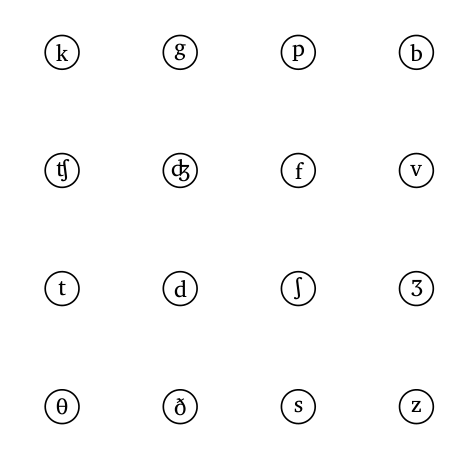
\includegraphics[width=0.5\textwidth]{img/classes-0.png}
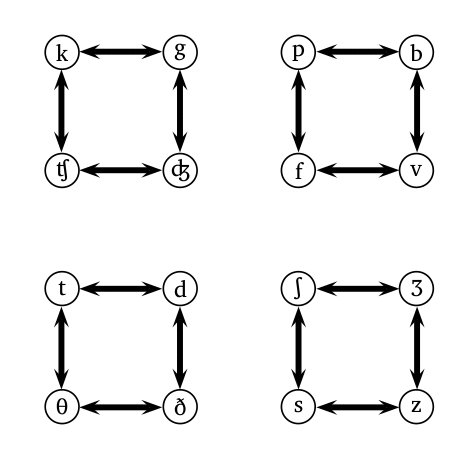
\includegraphics[width=0.5\textwidth]{img/classes-1.png}
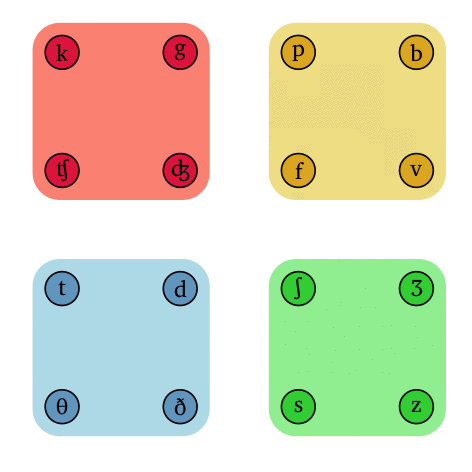
\includegraphics[width=0.5\textwidth]{img/classes-2.png}
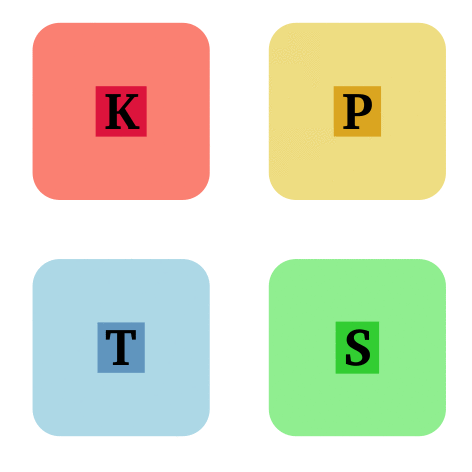
\includegraphics[width=0.5\textwidth]{img/classes-3.png}




\par\noindent\textbf{Dolgopolskys Lautklassenmodell}

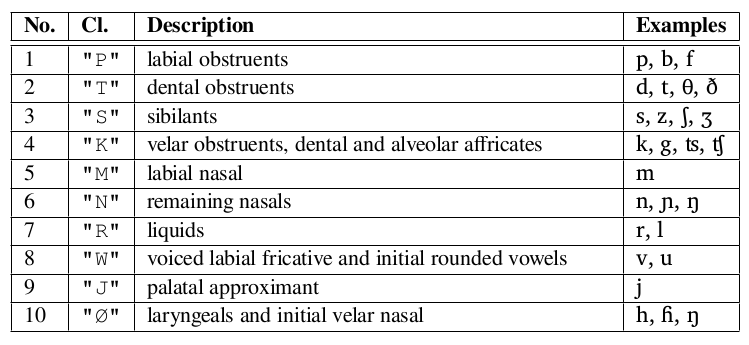
\includegraphics[width=\textwidth]{img/dolgo.png}



\par\noindent\textbf{Erweitertes Lautklassenmodell
(\href{http://bibliography.lingpy.org?key=List2014d}{List 2014})}

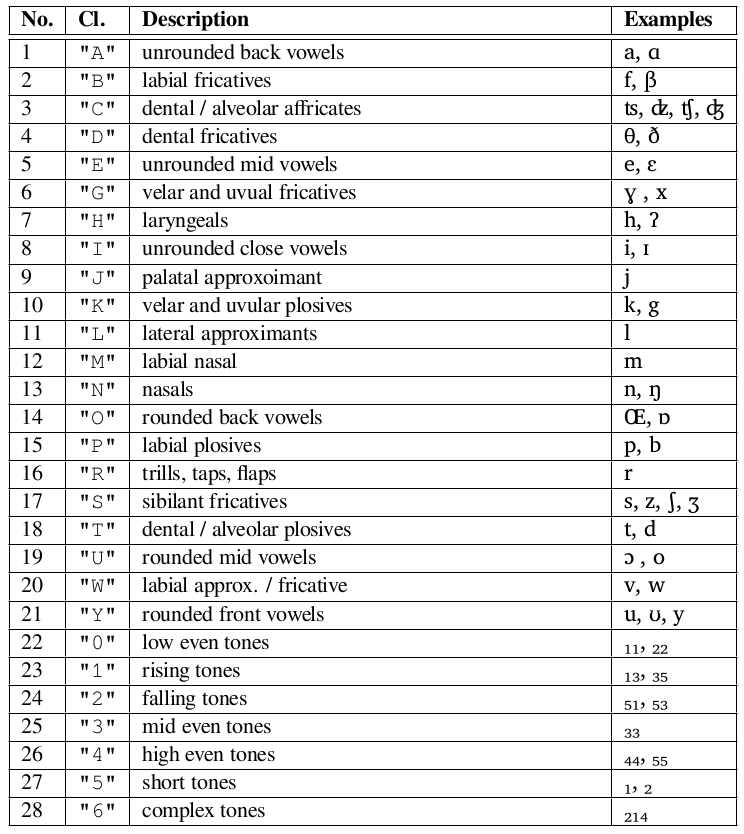
\includegraphics[width=\textwidth]{img/sca.png}


\subsubsection{\texorpdfstring{{Lautklassenkonvertierung mit
Python}}{Lautklassenkonvertierung mit Python}}

\par\noindent\textbf{Grundlegende Idee}

\begin{itemize}
\itemsep1pt\parskip0pt\parsep0pt
\item
  Um eine Sequenz in Lautklassen zu konvertieren, müssen wir für jeden
  möglichen Lautbuchstaben den entsprechenden Lautklassenbuchstaben
  definieren.
\item
  Am besten dafür geeignet ist ein Python-Dictionary, welches aus
  Key-Value-Paaren besteht und zu jedem Key den Value liefern kann.
\item
  Das Erstellen eines solchen Dictionaries ist zwar nervig, es ist aber
  die einfachste Möglichkeit, um nachher ein Wort zu konvertieren.
\item
  Das Wort muss allerdings segmentiert vorliegen, da wir ansonsten keine
  Möglichkeit haben, zu wissen, was jeweils ein Laut sein soll (vgl.
  Laute wie {[}tʰ{]} oder {[}t͡s{]}, die aus zwei oder mehr Zeichen
  bestehen).
\end{itemize}




\par\noindent\textbf{Workflow}

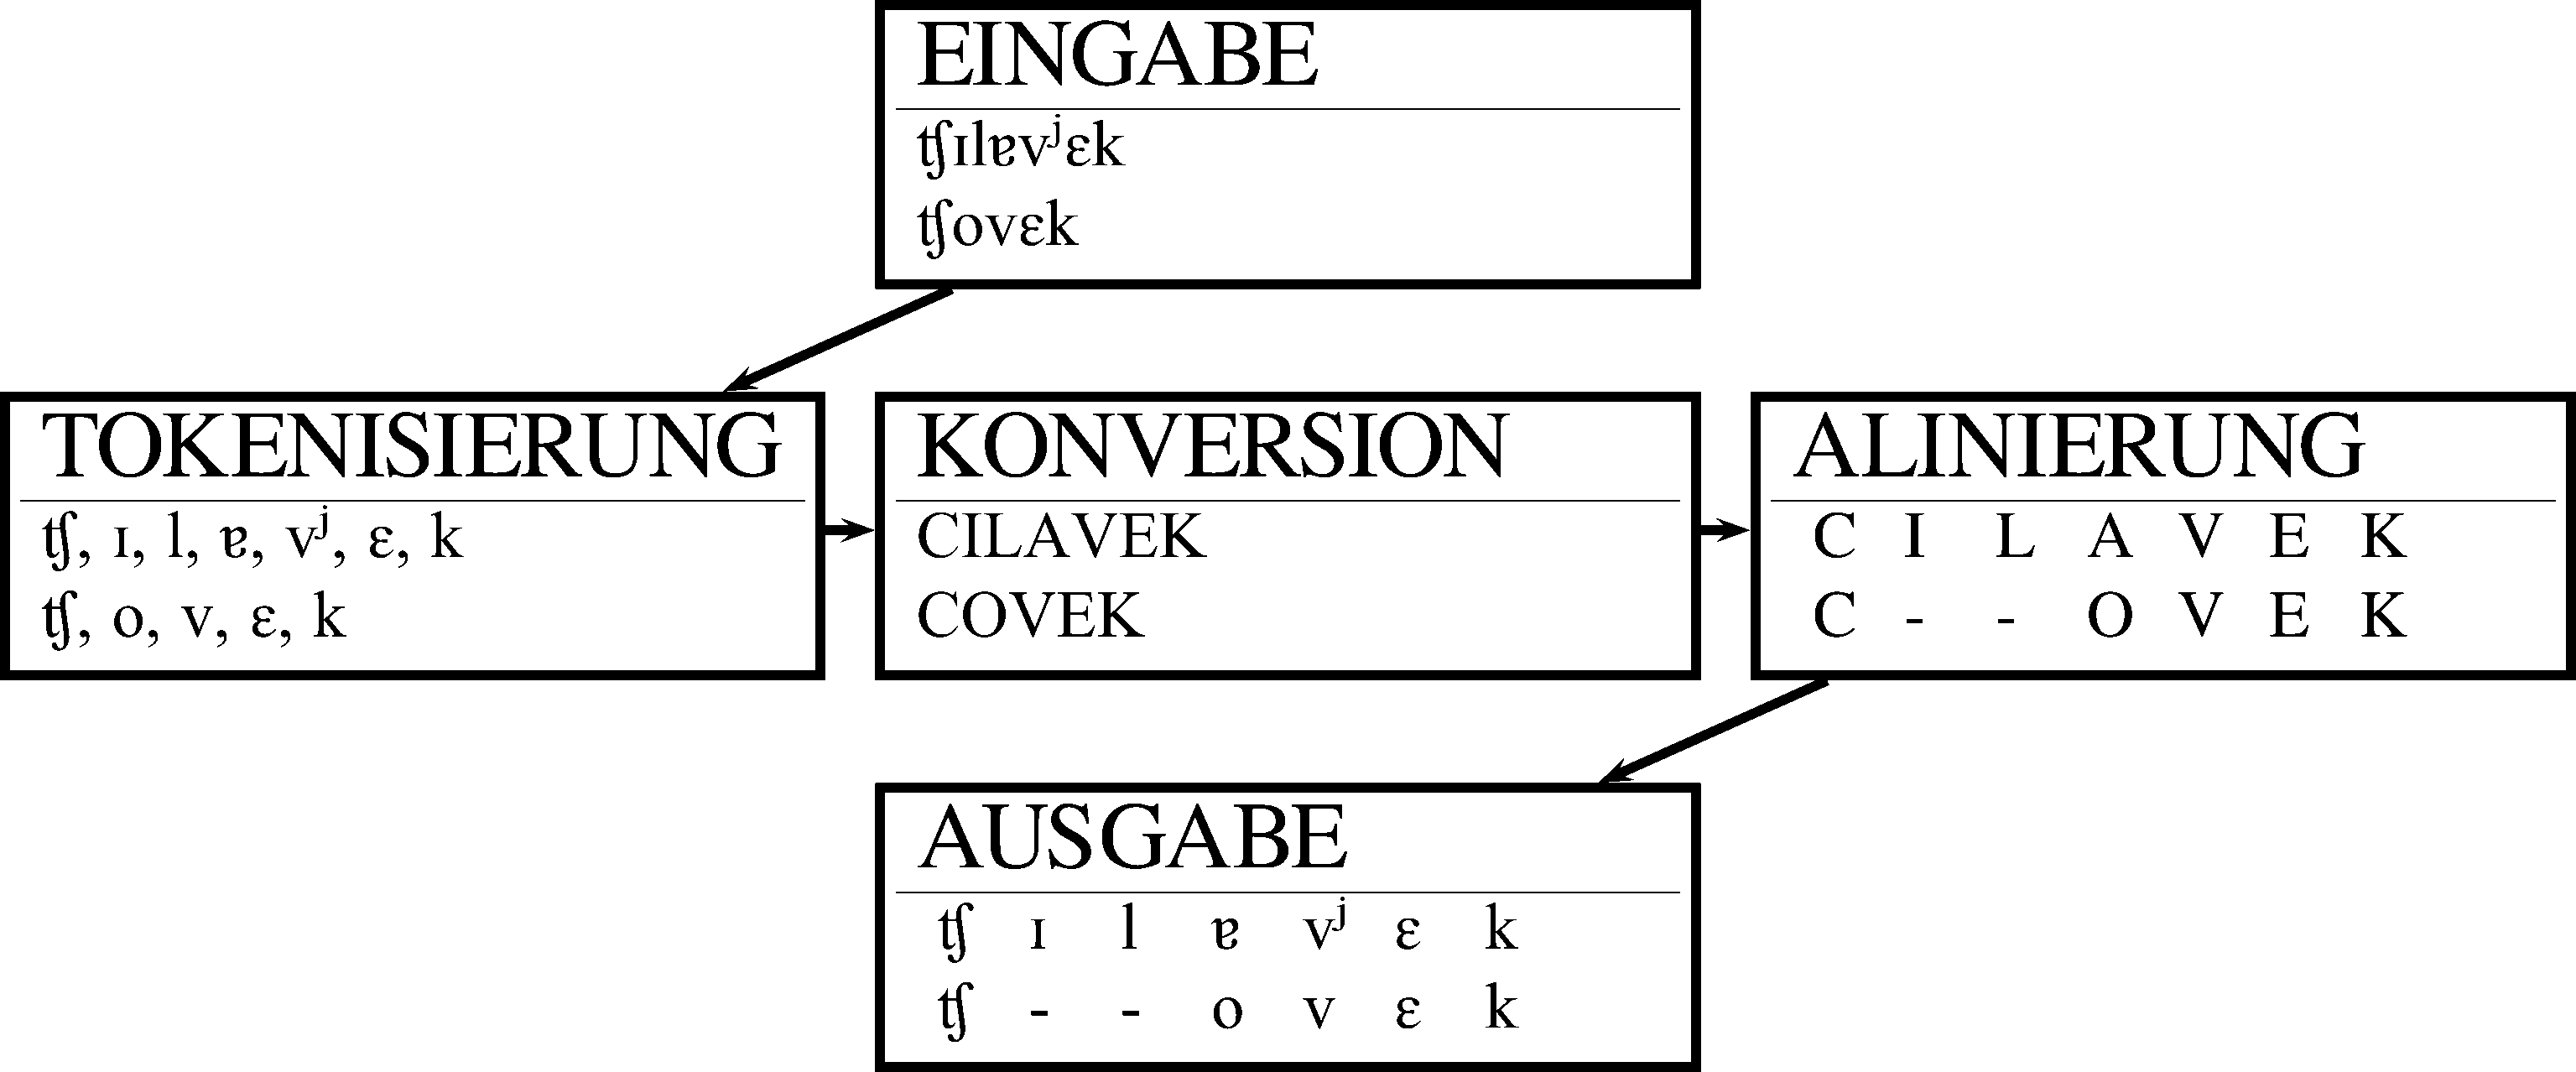
\includegraphics[width=\textwidth]{img/sca_workflow-4.png}


\par\noindent\textbf{Segmentierung}

Für die Segmentierung bedienen wir uns eines einfachen Modells: Jede
Sequenz wird mit Hilfe des Leerzeichens segmentiert dargestellt:

\begin{itemize}
\itemsep1pt\parskip0pt\parsep0pt
\item
  \emph{Tochter}: ``tʰɔxtʰər'' → ``tʰ ɔ x tʰ ə r''
\item
  \emph{daughter}: ``dɔːtʰər'' → ``d ɔː tʰ ə r''
\end{itemize}

Mit Python können wir diesen Input ganz schnell in eine Liste umwandeln:

\begin{verbatim}
>>> my_string = "tʰ ɔ x tʰ ə r"
>>> my_sequence = my_string.split(" ")
>>> my_sequence
['tʰ', 'ɔ', 'x', 'tʰ', 'ə', 'r']
\end{verbatim}




\par\noindent\textbf{Umwandlung}

Bei der Umwandlung mit Hilfe eines Dictionaries sollten wir damit
rechnen, dass bestimmte Zeichen nicht vorhanden sind (es gibt so viele
Symbole, und es kann fast unmöglich sein, alle zu finden, außerdem
können die Daten auch Fehler enthalten). Daher führen wir einen
dreistufigen Test ein.

\begin{verbatim}
def segment2class(segment, converter):
    """
    Convert a segment to a sound-class schema.
    """
    # erster versuch
    try:
        return converter[segment]
    except KeyError:
        # zweiter versuch
        try:
            return converter[segment[0]]
        except KeyError:
            # ansonsten, gib den "misserfolg"-character zurück
            return '0' 
\end{verbatim}



\subsubsection{Implementierung}

\par\noindent\textbf{Laden des Lautklassenmodells}

Wir speichern und laden den Converter
(\href{https://github.com/LinguList/pyjs-seminar/blob/master/website/code/dolgo.json}{dolgo.json})
im \href{http://de.wikipedia.org/wiki/json}{json-Format}, welches zu
einem der gängigsten Austauschformate geworden ist. Wir laden die Datei
mit Hilfe des \textbf{json}-Modules, wo uns automatisch ein
Python-Dictionary zurückgegeben wird.

\begin{verbatim}
def load_model(model):
    """
    Load the converter for a sound-class model.
    """
    # load the converter with json
    converter = json.load(open(model+'.json'))
    return converter
\end{verbatim}





\par\noindent\textbf{Lautklassenkonvertierung}

Die Konvertierung lässt sich mit sehr wenigen Zeilen Kode umsetzen, da
wir hier von der Listengenerationssyntax in Python Gebrauch machen
können (sogenannte
\href{http://www.secnetix.de/olli/Python/list_comprehensions.hawk}{list
comprehension}):

\begin{verbatim}
def segments2classes(segments, converter):
    """
    Convert a sound string to a sound-class string.
    """
    # check for segmented string
    if type(segments) == str:
        segments = segments.split(' ')
    # convert the segments
    classes = [segment2class(x) for x in segments]
    return classes
\end{verbatim}





\par\noindent\textbf{Rückkonvertierung}

Zur Rückkonvertierung brauchen wir den ursprünglichen String. Wir gehen
ja davon aus, dass wir die Strings zuerst in Lautklassen umwandeln,
diese dann alinieren, und nachher alles zurückkonvertieren. Hierbei
müssen wir im Prinzip nur merken, wo die Gaps eingesetzt wurden, wir
müssen also die Gaps aus der Lautklassensequenz in die ursprüngliche
Sequenz übertragen:

\begin{verbatim}
def classes2segments(classes, segments):
    """
    Convert an aligned string of sound classes back to the string of segments.
    """
    idx = len(segments)-1
    out = []
    for i in range(len(classes)-1,-1,-1):
        print(i,classes[i])
        if classes[i] == '-':
            out += [classes[i]]
        else:
            out += [segments[idx]]
            idx -= 1  
    return out[::-1] 
\end{verbatim}





\par\noindent\textbf{Vollständige Lautklassenbasierte Alinierung}

\begin{verbatim}
def sca_align(stringA, stringB, model="dolgo"):
    """
    Carry out sound-class based alignment analysis.
    """
    # check for strings passed as such 
    if type(stringA) == str:
        stringA = stringA.split(' ')
        stringB = stringB.split(' ')
    # load the converter
    converter = load_model(model)
    # Konvertierung
    seqA = segments2classes(stringA, converter)
    seqB = segments2classes(stringB, converter)
    # Alinierung
    almA, almB, ED = wf_align(seqA, seqB)
    # Rück-Konvertierung
    outA = classes2segments(almA, stringA)
    outB = classes2segments(almB, stringB)
    return outA, outB, ED
\end{verbatim}


\subsection{Phonetische Alinierung mit LingPy}
\subsubsection{\texorpdfstring{{Was ist LingPy?}}{Was ist LingPy?}}

\par\noindent\textbf{Grundlegendes zu LingPy}

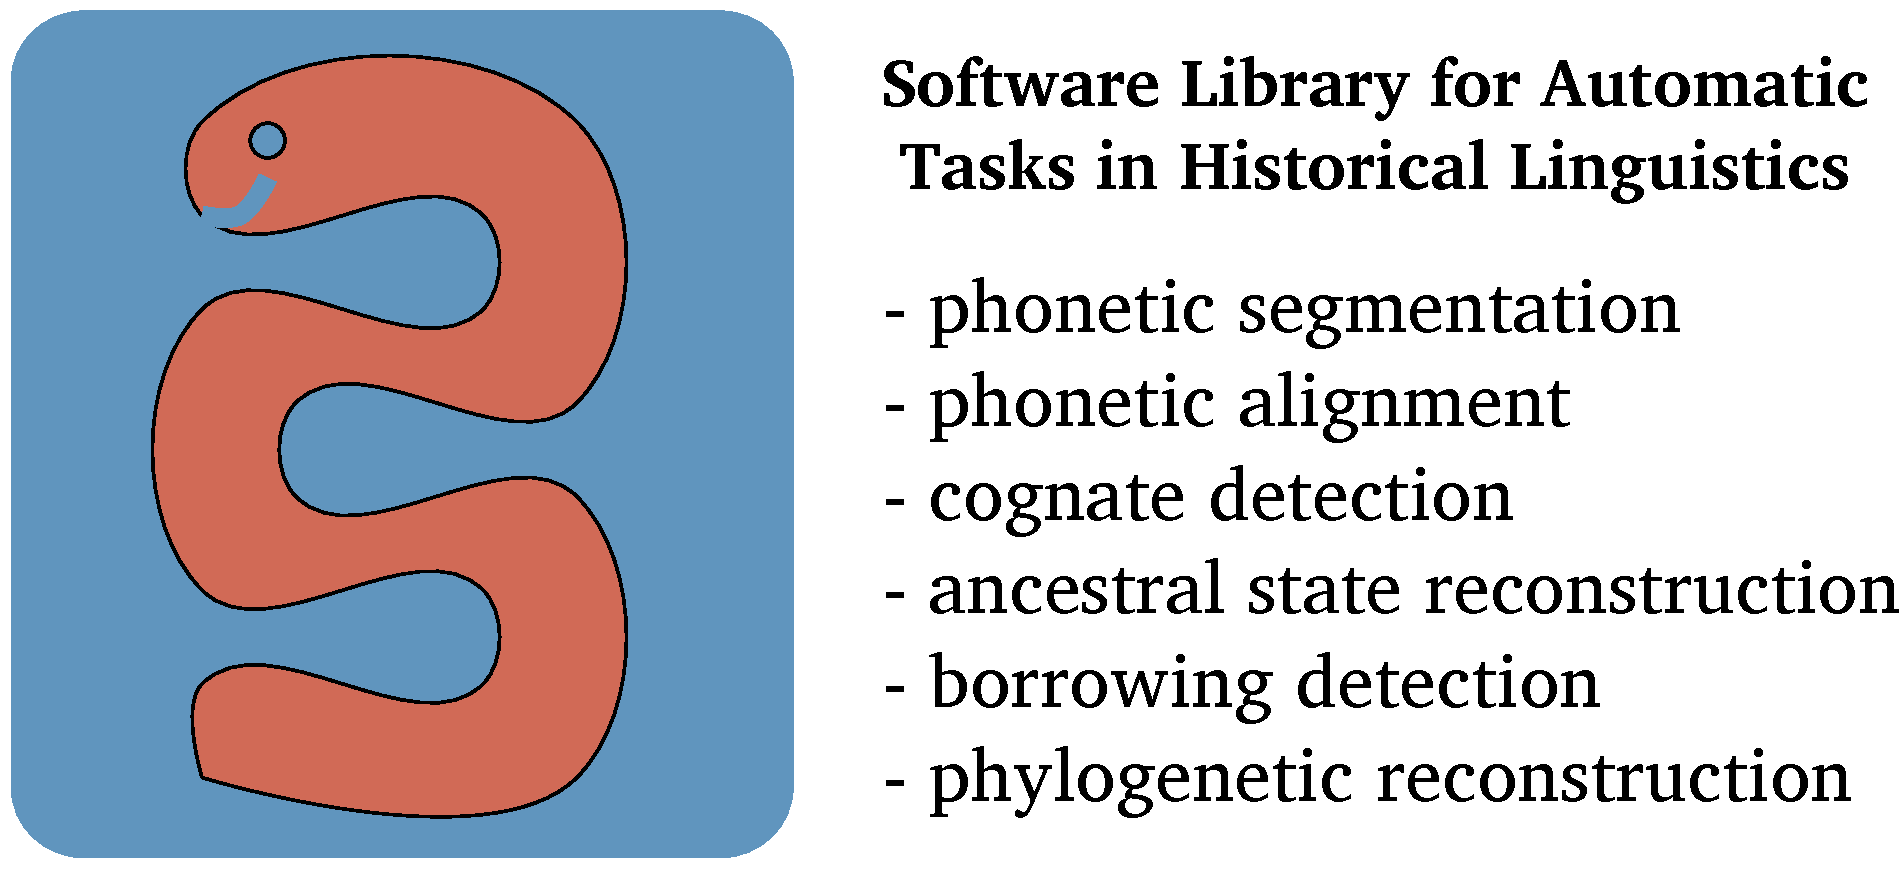
\includegraphics[width=\textwidth]{img/lingpy.pdf}






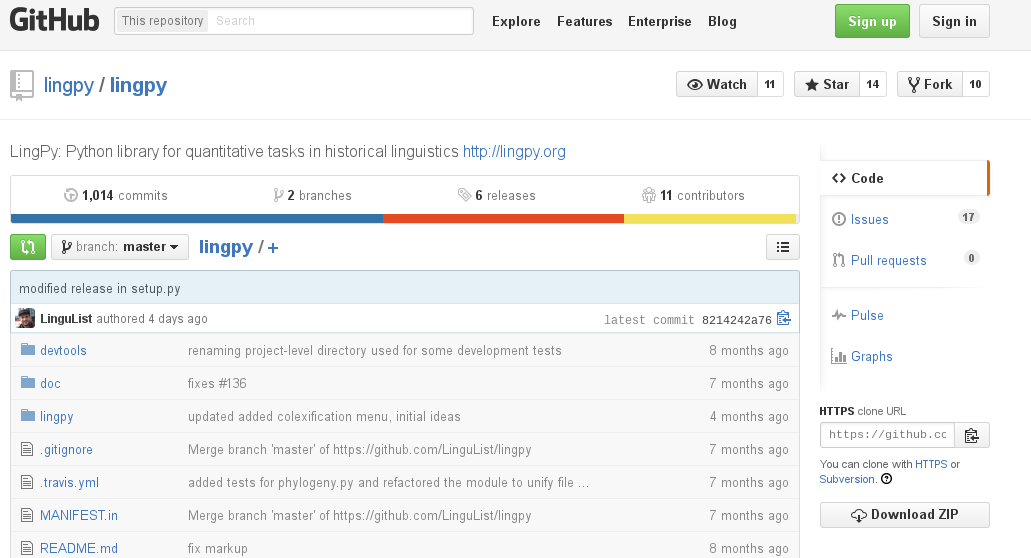
\includegraphics[width=\textwidth]{img/lingpy-git.png}


\subsubsection{\texorpdfstring{{Grundlegende
Befehle}}{Grundlegende Befehle}}

\par\noindent\textbf{Arbeiten mit Sequenzen}

\begin{verbatim}
>>> from lingpy import *
>>> seq = sampa2uni('t_hOxt_h@r')
>>> seq
'tʰɔxtʰər'
>>> tokens = ipa2tokens(seq)
>>> tokens
['tʰ', 'o', 'x', 't', 'ə', 'r']
>>> classes = tokens2class(tokens, 'sca')
>>> classes
['T', 'U', 'G', 'T', 'E', 'R']
>>> classes = tokens2class(tokens, 'dolgo')
>>> classes
['T', 'V', 'K', 'T', 'V', 'R']
>>> from lingpy.sequence.sound_classes import *
>>> syllabify(seq)
['tʰ', 'ɔ', 'x', '◦', 'tʰ', 'ə', 'r']
\end{verbatim}




\par\noindent\textbf{Vergleichen von Sequenzen}

\begin{verbatim}
>>> seq1 = ipa2tokens(sampa2uni('t_hOxt_h@r'))
>>> seq2 = ipa2tokens('dɔːtʰər')
>>> seq3 = ipa2tokens('dɔttər')
>>> edit_dist(seq1, seq2)
3
>>> nw_align(seq1,seq2)
(['tʰ', 'ɔ', 'x', 'tʰ', 'ə', 'r'], ['-', 'd', 'ɔː', 'tʰ', 'ə', 'r'], 0.0)
>>> sw_align(seq1, seq2)
((['tʰ', 'ɔ', 'x'], ['tʰ', 'ə', 'r'], []), (['d', 'ɔː'], ['tʰ', 'ə', 'r'], []), 3.0)
>>> we_align(seq1,seq2)
[(['tʰ', 'ə', 'r'], ['tʰ', 'ə', 'r'], 3.0)]
>>> mult_align([seq1,seq2,seq3],pprint=True)
tʰ  ɔ   x   tʰ  ə   r
d   ɔː  -   tʰ  ə   r
d   ɔ   -   tt  ə   r
\end{verbatim}



\subsubsection{\texorpdfstring{{Workflows}}{Workflows}}

\par\noindent\textbf{Grundlegendes vorweg}

Mit LingPy lassen sich gezielt Daten im großen Stil analysieren. Dafür
braucht man einen Workflow, und man schreibt dann normalerweise ein
kleines Skript, mit dessen Hilfe sich die Berechnungen (zum Beispiel die
Alinierung von 100 verschiedenen Wortlisten) in einem ``Rutsch''
erledigen lassen.

In dieser Sitzung werde ich nur einen kleinen Teil eines Workflows
vorstellen, und zwar die Möglichkeit, eine Alinierung automatisch
vorzunehmen.




\par\noindent\textbf{Das Input-Format}

Das Input-Format für Alinierungen in Textdateien ist relativ einfach:

\begin{itemize}
\itemsep1pt\parskip0pt\parsep0pt
\item
  die erste Zeile enthält einen Verweis auf den Datensatz
\item
  die zweite Zeile enthält einen Verweis auf die Gruppe von Wörter, die
  aliniert werden sollen
\item
  die folgenden Zeilen enthalten nun, separiert durch einen Tabstop, den
  Namen der Sprache und die Daten in IPA.
\item
  wer seine Daten vorsegmentieren will, kann das tun und einfach einen
  String durch Leertasten separieren, alternativ kann man das auch von
  LingPy automatisch übernehmen lassen
\end{itemize}




\par\noindent\textbf{Das Input-Format: Beispiel}

\begin{verbatim}
French
French \*le chasseur\* (< Latin \*captiatore\*), Chart 447
Chevroux..........    ʦ a ʃ ɑː
Vaugondry.........    ʦ a ʃ ø
L'Auberson........    ʧ a s ø
Vallorbe..........    ʧ a ʃ oː
Le Sentier........    ʦ a ʃ au
Longirod..........    ʦ a f j aː
Commugny..........    θ ɛ f j œi
Vullierens........    ʧ a s ɑː
Arnex.............    ʧ a ʃ au
Villars-le-Terroir    ʦ a ʃ aː
Prahins...........    ʦ a ʃ ɔː
Montpreveyres.....    ʦ a ʃ ɑː
Charnex...........    ʦ e ç æ͜u
Roche.............    ʦ a ç øː
Ormont-Dessus.....    ʦ a ɬ au
Château-d'Oex.....    ʦ a ç au
St-Gingolph.......    ʦ a f j au
Collombey.........    ʦ a f j œi
Champéry..........    ʦ a ç œː
Martigny..........    ʦ a f j œi
Orsières..........    ʦ a s j ɜu
Lourtier..........    ʦ a ç ɔː
Fully.............    ʦ a ç œu
Conthey...........    ʦ a θ j œi
Nendaz............    ʧ a ʃ ç ɜu
Savièse...........    ʦ a s j u
Ayent.............    ʦ a ç øi
Miège.............    ʦ a s j ou
Grône.............    ʦ a ʃ ç ou k
Évolène...........    ʦ a ʃ j ou
Grimentz..........    ʦ a s j ou
Collex............    θ e f j ø
Vernier...........    θ ɛ f j ø
Laconnex..........    θ ɛ f j œ
Veyrier...........    θ ɛ f j ø
Hermance..........    θ ɛ f j œ
Semsalves.........    ʦ a ç a
Montbovon.........    ʦ a ç aː
Arconciel.........    ʦ a ç aː
Avry-sur-Matran...    ʦ a ç j aː
Courtepin.........    ʦ a ç aː
Dompierre.........    ʦ a ç aː
Murist............    ʦ a ç aː
Sugiez............    ʧ æ ʃ ɔ
Montalchez........    ʦ a ʃ a
Boudry............    ʦ a s œː r
Corcelles.........    ʧ a s y
Landeron..........    ʧ a s eː r
Savagnier.........    ʧ a s øː r
Côte-aux-Fées.....    ʦ a ʃ œ
Noiraigue.........    ʧ a ʃ œ
Chaux-du-Milieu...    ʧ a s y
Cerneux-Péquignot.    ʧ ɛ s u
Lamboing..........    ʧ a s œ
Orvin.............    ʧ s u
Plagne............    ʧ s u
Sombeval..........    ʧ s u
Court.............    ʧ s u
Vermes............    ʧ s u
Develier..........    ʧ ə s u
Cerlatez..........    ʧ æ s u
Courtedoux........    ʧ s u
\end{verbatim}



\par\noindent\textbf{Der Alinierungsworkflow: Multiple Alinierung}

\begin{verbatim}
>>> from lingpy import *
>>> msa = Multiple('data/french-chasseur.msq')
>>> msa.prog_align()
>>> print(msa)
ʦ   a   ʃ   -   ɑː  -
ʦ   a   ʃ   -   ø   -
ʧ   a   s   -   ø   -
ʧ   a   ʃ   -   oː  -
ʦ   a   ʃ   -   au  -
ʦ   a   f   j   aː  -
θ   ɛ   f   j   œi  -
ʧ   a   s   -   ɑː  -
ʧ   a   ʃ   -   au  -
ʦ   a   ʃ   -   aː  -
ʦ   a   ʃ   -   ɔː  -
ʦ   a   ʃ   -   ɑː  -
ʦ   e   ç   -   æ͜u -
ʦ   a   ç   -   øː  -
ʦ   a   ɬ   -   au  -
ʦ   a   ç   -   au  -
ʦ   a   f   j   au  -
ʦ   a   f   j   œi  -
ʦ   a   ç   -   œː  -
ʦ   a   f   j   œi  -
ʦ   a   s   j   ɜu  -
ʦ   a   ç   -   ɔː  -
ʦ   a   ç   -   œu  -
ʦ   a   θ   j   œi  -
ʧ   a   ʃ   ç   ɜu  -
ʦ   a   s   j   u   -
ʦ   a   ç   -   øi  -
ʦ   a   s   j   ou  -
ʦ   a   ʃ   ç   ou  k
ʦ   a   ʃ   j   ou  -
ʦ   a   s   j   ou  -
θ   e   f   j   ø   -
θ   ɛ   f   j   ø   -
θ   ɛ   f   j   œ   -
θ   ɛ   f   j   ø   -
θ   ɛ   f   j   œ   -
ʦ   a   ç   -   a   -
ʦ   a   ç   -   aː  -
ʦ   a   ç   -   aː  -
ʦ   a   ç   j   aː  -
ʦ   a   ç   -   aː  -
ʦ   a   ç   -   aː  -
ʦ   a   ç   -   aː  -
ʧ   æ   ʃ   -   ɔ   -
ʦ   a   ʃ   -   a   -
ʦ   a   s   -   œː  r
ʧ   a   s   -   y   -
ʧ   a   s   -   eː  r
ʧ   a   s   -   øː  r
ʦ   a   ʃ   -   œ   -
ʧ   a   ʃ   -   œ   -
ʧ   a   s   -   y   -
ʧ   ɛ   s   -   u   -
ʧ   a   s   -   œ   -
ʧ   -   s   -   u   -
ʧ   -   s   -   u   -
ʧ   -   s   -   u   -
ʧ   -   s   -   u   -
ʧ   -   s   -   u   -
ʧ   ə   s   -   u   -
ʧ   æ   s   -   u   -
ʧ   -   s   -   u   -
\end{verbatim}


\par\noindent\textbf{Der Alinierungsworkflow: Output}

\begin{verbatim}
>>> msa.output('msa', filename='data/french-chasseur')
>>> msa.output('html', filename='data/french-chasseur')
>>> msa.output('tex', filename='data/french-chasseur')
\end{verbatim}



\par\noindent\textbf{Der Alinierungsworkflow: Ergebnisse (HTML-Output)}


\par\noindent\textbf{Der Alinierungsworkflow: Ergebnisse (LaTeX-Output)}

\begin{verbatim}
\documentclass[xetex,12pt]{scrartcl}
\usepackage{xltxtra,polyglossia,color,colortbl}
\usepackage{pspicture,pst-node,xcolor}
\usepackage{geometry}
\usepackage{array}

\setmainfont[Mapping=tex-text,Scale=1.0]{Charis SIL}
\setsansfont[Mapping=tex-text,Scale=1.0]{FreeSans}
\setmonofont{DejaVu Sans Mono}

\setmainlanguage{english}

% set the new font width, declare the new lengths first
\newlength\MyWidth
\newlength\MyHeight
% set the new lengths
\setlength\MyWidth{13.500000cm} % hier die Breite eintragen
\setlength\MyHeight{32.000000cm} % hier die Höhe eintragen

% set new lengths to put the picture
\newlength\MyWput
\newlength\MyHput
\setlength\MyWput{\MyWidth}
\setlength\MyHput{\MyHeight}
% calculate the values by dividing etc.
\divide\MyWput by 2
\divide\MyHput by 2
\addtolength\MyHput{-\MyHeight}
\addtolength\MyHput{10 pt}
\makeatletter
\addtolength\MyHput{\@ptsize pt}
\makeatother

\geometry{papersize={\MyWidth,\MyHeight},total={\MyWidth,\MyHeight}}

\parindent 0pt
\begin{document}\thispagestyle{empty}

% define the colors
%\definecolor{colV}{HTML}{C86464} 
%\definecolor{colK}{HTML}{C89664} 
%\definecolor{colP}{HTML}{C8C864} 
%\definecolor{colH}{HTML}{96C864} 
%\definecolor{colJ}{HTML}{64C864} 
%\definecolor{colM}{HTML}{64C896} 
%\definecolor{colN}{HTML}{64C8C8} 
%\definecolor{colS}{HTML}{6496C8} 
%\definecolor{colR}{HTML}{6464C8} 
%\definecolor{colT}{HTML}{9664C8} 
%\definecolor{colW}{HTML}{C864C8} 
%\definecolor{col1}{HTML}{C86496} 
%\definecolor{col2}{HTML}{BBBBBB}
%\definecolor{colX}{HTML}{C0C0C0}

\definecolor{colV}{HTML}{808080} 
\definecolor{colK}{HTML}{F2F2F2} 
\definecolor{colP}{HTML}{E6E6E6} 
\definecolor{colH}{HTML}{B2B2B2} 
\definecolor{colJ}{HTML}{999999} 
\definecolor{colM}{HTML}{BFBFBF} 
\definecolor{colN}{HTML}{BFBFBF} 
\definecolor{colS}{HTML}{CCCCCC} 
\definecolor{colR}{HTML}{A6A6A6} 
\definecolor{colT}{HTML}{D9D9D9} 
\definecolor{colW}{HTML}{8C8C8C} 
\definecolor{col1}{HTML}{FFFFFF} 
\definecolor{col2}{HTML}{737373}
\definecolor{colX}{HTML}{FFFFFF}

\rput(\MyWput,\MyHput){%
\pspicture[showgrid=false](0,0)(\the\MyWidth,\the\MyHeight)
% Insert your Code here, as you like! Coordinate system starts with 0,0 on the left bottom of the
% page. 
\rput(6.75,15.75){%
\tabular{lcccccc}
\bf\ttfamily Taxon & \multicolumn{6}{l}{\bf\ttfamily Alignment}\\
\ttfamily Chevroux&\cellcolor{colK}ʦ&\cellcolor{colV}a&\cellcolor{colS}ʃ&\cellcolor{colX}-&\cellcolor{colV}ɑː&\cellcolor{colX}-\\
\ttfamily Vaugondry&\cellcolor{colK}ʦ&\cellcolor{colV}a&\cellcolor{colS}ʃ&\cellcolor{colX}-&\cellcolor{colV}ø&\cellcolor{colX}-\\
\ttfamily L'Auberson&\cellcolor{colK}ʧ&\cellcolor{colV}a&\cellcolor{colS}s&\cellcolor{colX}-&\cellcolor{colV}ø&\cellcolor{colX}-\\
\ttfamily Vallorbe&\cellcolor{colK}ʧ&\cellcolor{colV}a&\cellcolor{colS}ʃ&\cellcolor{colX}-&\cellcolor{colV}oː&\cellcolor{colX}-\\
\ttfamily Le Sentier&\cellcolor{colK}ʦ&\cellcolor{colV}a&\cellcolor{colS}ʃ&\cellcolor{colX}-&\cellcolor{colV}au&\cellcolor{colX}-\\
\ttfamily Longirod&\cellcolor{colK}ʦ&\cellcolor{colV}a&\cellcolor{colP}f&\cellcolor{colJ}j&\cellcolor{colV}aː&\cellcolor{colX}-\\
\ttfamily Commugny&\cellcolor{colT}θ&\cellcolor{colV}ɛ&\cellcolor{colP}f&\cellcolor{colJ}j&\cellcolor{colV}œi&\cellcolor{colX}-\\
\ttfamily Vullierens&\cellcolor{colK}ʧ&\cellcolor{colV}a&\cellcolor{colS}s&\cellcolor{colX}-&\cellcolor{colV}ɑː&\cellcolor{colX}-\\
\ttfamily Arnex&\cellcolor{colK}ʧ&\cellcolor{colV}a&\cellcolor{colS}ʃ&\cellcolor{colX}-&\cellcolor{colV}au&\cellcolor{colX}-\\
\ttfamily Villars-le-Terroir&\cellcolor{colK}ʦ&\cellcolor{colV}a&\cellcolor{colS}ʃ&\cellcolor{colX}-&\cellcolor{colV}aː&\cellcolor{colX}-\\
\ttfamily Prahins&\cellcolor{colK}ʦ&\cellcolor{colV}a&\cellcolor{colS}ʃ&\cellcolor{colX}-&\cellcolor{colV}ɔː&\cellcolor{colX}-\\
\ttfamily Montpreveyres&\cellcolor{colK}ʦ&\cellcolor{colV}a&\cellcolor{colS}ʃ&\cellcolor{colX}-&\cellcolor{colV}ɑː&\cellcolor{colX}-\\
\ttfamily Charnex&\cellcolor{colK}ʦ&\cellcolor{colV}e&\cellcolor{colS}ç&\cellcolor{colX}-&\cellcolor{colV}æ͜u&\cellcolor{colX}-\\
\ttfamily Roche&\cellcolor{colK}ʦ&\cellcolor{colV}a&\cellcolor{colS}ç&\cellcolor{colX}-&\cellcolor{colV}øː&\cellcolor{colX}-\\
\ttfamily Ormont-Dessus&\cellcolor{colK}ʦ&\cellcolor{colV}a&\cellcolor{colR}ɬ&\cellcolor{colX}-&\cellcolor{colV}au&\cellcolor{colX}-\\
\ttfamily Château-d'Oex&\cellcolor{colK}ʦ&\cellcolor{colV}a&\cellcolor{colS}ç&\cellcolor{colX}-&\cellcolor{colV}au&\cellcolor{colX}-\\
\ttfamily St-Gingolph&\cellcolor{colK}ʦ&\cellcolor{colV}a&\cellcolor{colP}f&\cellcolor{colJ}j&\cellcolor{colV}au&\cellcolor{colX}-\\
\ttfamily Collombey&\cellcolor{colK}ʦ&\cellcolor{colV}a&\cellcolor{colP}f&\cellcolor{colJ}j&\cellcolor{colV}œi&\cellcolor{colX}-\\
\ttfamily Champéry&\cellcolor{colK}ʦ&\cellcolor{colV}a&\cellcolor{colS}ç&\cellcolor{colX}-&\cellcolor{colV}œː&\cellcolor{colX}-\\
\ttfamily Martigny&\cellcolor{colK}ʦ&\cellcolor{colV}a&\cellcolor{colP}f&\cellcolor{colJ}j&\cellcolor{colV}œi&\cellcolor{colX}-\\
\ttfamily Orsières&\cellcolor{colK}ʦ&\cellcolor{colV}a&\cellcolor{colS}s&\cellcolor{colJ}j&\cellcolor{colV}ɜu&\cellcolor{colX}-\\
\ttfamily Lourtier&\cellcolor{colK}ʦ&\cellcolor{colV}a&\cellcolor{colS}ç&\cellcolor{colX}-&\cellcolor{colV}ɔː&\cellcolor{colX}-\\
\ttfamily Fully&\cellcolor{colK}ʦ&\cellcolor{colV}a&\cellcolor{colS}ç&\cellcolor{colX}-&\cellcolor{colV}œu&\cellcolor{colX}-\\
\ttfamily Conthey&\cellcolor{colK}ʦ&\cellcolor{colV}a&\cellcolor{colT}θ&\cellcolor{colJ}j&\cellcolor{colV}œi&\cellcolor{colX}-\\
\ttfamily Nendaz&\cellcolor{colK}ʧ&\cellcolor{colV}a&\cellcolor{colS}ʃ&\cellcolor{colS}ç&\cellcolor{colV}ɜu&\cellcolor{colX}-\\
\ttfamily Savièse&\cellcolor{colK}ʦ&\cellcolor{colV}a&\cellcolor{colS}s&\cellcolor{colJ}j&\cellcolor{colV}u&\cellcolor{colX}-\\
\ttfamily Ayent&\cellcolor{colK}ʦ&\cellcolor{colV}a&\cellcolor{colS}ç&\cellcolor{colX}-&\cellcolor{colV}øi&\cellcolor{colX}-\\
\ttfamily Miège&\cellcolor{colK}ʦ&\cellcolor{colV}a&\cellcolor{colS}s&\cellcolor{colJ}j&\cellcolor{colV}ou&\cellcolor{colX}-\\
\ttfamily Grône&\cellcolor{colK}ʦ&\cellcolor{colV}a&\cellcolor{colS}ʃ&\cellcolor{colS}ç&\cellcolor{colV}ou&\cellcolor{colK}k\\
\ttfamily Évolène&\cellcolor{colK}ʦ&\cellcolor{colV}a&\cellcolor{colS}ʃ&\cellcolor{colJ}j&\cellcolor{colV}ou&\cellcolor{colX}-\\
\ttfamily Grimentz&\cellcolor{colK}ʦ&\cellcolor{colV}a&\cellcolor{colS}s&\cellcolor{colJ}j&\cellcolor{colV}ou&\cellcolor{colX}-\\
\ttfamily Collex&\cellcolor{colT}θ&\cellcolor{colV}e&\cellcolor{colP}f&\cellcolor{colJ}j&\cellcolor{colV}ø&\cellcolor{colX}-\\
\ttfamily Vernier&\cellcolor{colT}θ&\cellcolor{colV}ɛ&\cellcolor{colP}f&\cellcolor{colJ}j&\cellcolor{colV}ø&\cellcolor{colX}-\\
\ttfamily Laconnex&\cellcolor{colT}θ&\cellcolor{colV}ɛ&\cellcolor{colP}f&\cellcolor{colJ}j&\cellcolor{colV}œ&\cellcolor{colX}-\\
\ttfamily Veyrier&\cellcolor{colT}θ&\cellcolor{colV}ɛ&\cellcolor{colP}f&\cellcolor{colJ}j&\cellcolor{colV}ø&\cellcolor{colX}-\\
\ttfamily Hermance&\cellcolor{colT}θ&\cellcolor{colV}ɛ&\cellcolor{colP}f&\cellcolor{colJ}j&\cellcolor{colV}œ&\cellcolor{colX}-\\
\ttfamily Semsalves&\cellcolor{colK}ʦ&\cellcolor{colV}a&\cellcolor{colS}ç&\cellcolor{colX}-&\cellcolor{colV}a&\cellcolor{colX}-\\
\ttfamily Montbovon&\cellcolor{colK}ʦ&\cellcolor{colV}a&\cellcolor{colS}ç&\cellcolor{colX}-&\cellcolor{colV}aː&\cellcolor{colX}-\\
\ttfamily Arconciel&\cellcolor{colK}ʦ&\cellcolor{colV}a&\cellcolor{colS}ç&\cellcolor{colX}-&\cellcolor{colV}aː&\cellcolor{colX}-\\
\ttfamily Avry-sur-Matran&\cellcolor{colK}ʦ&\cellcolor{colV}a&\cellcolor{colS}ç&\cellcolor{colJ}j&\cellcolor{colV}aː&\cellcolor{colX}-\\
\ttfamily Courtepin&\cellcolor{colK}ʦ&\cellcolor{colV}a&\cellcolor{colS}ç&\cellcolor{colX}-&\cellcolor{colV}aː&\cellcolor{colX}-\\
\ttfamily Dompierre&\cellcolor{colK}ʦ&\cellcolor{colV}a&\cellcolor{colS}ç&\cellcolor{colX}-&\cellcolor{colV}aː&\cellcolor{colX}-\\
\ttfamily Murist&\cellcolor{colK}ʦ&\cellcolor{colV}a&\cellcolor{colS}ç&\cellcolor{colX}-&\cellcolor{colV}aː&\cellcolor{colX}-\\
\ttfamily Sugiez&\cellcolor{colK}ʧ&\cellcolor{colV}æ&\cellcolor{colS}ʃ&\cellcolor{colX}-&\cellcolor{colV}ɔ&\cellcolor{colX}-\\
\ttfamily Montalchez&\cellcolor{colK}ʦ&\cellcolor{colV}a&\cellcolor{colS}ʃ&\cellcolor{colX}-&\cellcolor{colV}a&\cellcolor{colX}-\\
\ttfamily Boudry&\cellcolor{colK}ʦ&\cellcolor{colV}a&\cellcolor{colS}s&\cellcolor{colX}-&\cellcolor{colV}œː&\cellcolor{colR}r\\
\ttfamily Corcelles&\cellcolor{colK}ʧ&\cellcolor{colV}a&\cellcolor{colS}s&\cellcolor{colX}-&\cellcolor{colV}y&\cellcolor{colX}-\\
\ttfamily Landeron&\cellcolor{colK}ʧ&\cellcolor{colV}a&\cellcolor{colS}s&\cellcolor{colX}-&\cellcolor{colV}eː&\cellcolor{colR}r\\
\ttfamily Savagnier&\cellcolor{colK}ʧ&\cellcolor{colV}a&\cellcolor{colS}s&\cellcolor{colX}-&\cellcolor{colV}øː&\cellcolor{colR}r\\
\ttfamily Côte-aux-Fées&\cellcolor{colK}ʦ&\cellcolor{colV}a&\cellcolor{colS}ʃ&\cellcolor{colX}-&\cellcolor{colV}œ&\cellcolor{colX}-\\
\ttfamily Noiraigue&\cellcolor{colK}ʧ&\cellcolor{colV}a&\cellcolor{colS}ʃ&\cellcolor{colX}-&\cellcolor{colV}œ&\cellcolor{colX}-\\
\ttfamily Chaux-du-Milieu&\cellcolor{colK}ʧ&\cellcolor{colV}a&\cellcolor{colS}s&\cellcolor{colX}-&\cellcolor{colV}y&\cellcolor{colX}-\\
\ttfamily Cerneux-Péquignot&\cellcolor{colK}ʧ&\cellcolor{colV}ɛ&\cellcolor{colS}s&\cellcolor{colX}-&\cellcolor{colV}u&\cellcolor{colX}-\\
\ttfamily Lamboing&\cellcolor{colK}ʧ&\cellcolor{colV}a&\cellcolor{colS}s&\cellcolor{colX}-&\cellcolor{colV}œ&\cellcolor{colX}-\\
\ttfamily Orvin&\cellcolor{colK}ʧ&\cellcolor{colX}-&\cellcolor{colS}s&\cellcolor{colX}-&\cellcolor{colV}u&\cellcolor{colX}-\\
\ttfamily Plagne&\cellcolor{colK}ʧ&\cellcolor{colX}-&\cellcolor{colS}s&\cellcolor{colX}-&\cellcolor{colV}u&\cellcolor{colX}-\\
\ttfamily Sombeval&\cellcolor{colK}ʧ&\cellcolor{colX}-&\cellcolor{colS}s&\cellcolor{colX}-&\cellcolor{colV}u&\cellcolor{colX}-\\
\ttfamily Court&\cellcolor{colK}ʧ&\cellcolor{colX}-&\cellcolor{colS}s&\cellcolor{colX}-&\cellcolor{colV}u&\cellcolor{colX}-\\
\ttfamily Vermes&\cellcolor{colK}ʧ&\cellcolor{colX}-&\cellcolor{colS}s&\cellcolor{colX}-&\cellcolor{colV}u&\cellcolor{colX}-\\
\ttfamily Develier&\cellcolor{colK}ʧ&\cellcolor{colV}ə&\cellcolor{colS}s&\cellcolor{colX}-&\cellcolor{colV}u&\cellcolor{colX}-\\
\ttfamily Cerlatez&\cellcolor{colK}ʧ&\cellcolor{colV}æ&\cellcolor{colS}s&\cellcolor{colX}-&\cellcolor{colV}u&\cellcolor{colX}-\\
\ttfamily Courtedoux&\cellcolor{colK}ʧ&\cellcolor{colX}-&\cellcolor{colS}s&\cellcolor{colX}-&\cellcolor{colV}u&\cellcolor{colX}-\\
&\color{white}XXX&\color{white}XXX&\color{white}XXX&\color{white}XXX&\color{white}XXX&\color{white}XXX\\
\endtabular

}
\endpspicture}
\end{verbatim}
\end{document}



